% =====================================================================
%  monoT5 Layer-Level Activation Patching — Full Experiment Report
%  Compile with:  pdflatex patching_experiment_report.tex  (run twice)
%  Figure paths are relative to this file (outputs/...), so compile
%  from the 01_monot5_layer_patching/ directory.
% =====================================================================
\documentclass[11pt]{article}

\usepackage[margin=1in]{geometry}
\usepackage{amsmath, amssymb}
\usepackage{graphicx}
\usepackage{booktabs}
\usepackage{longtable}
\usepackage{array}
\usepackage{float}
\usepackage{xcolor}
\usepackage{caption}
\usepackage{subcaption}
\usepackage{enumitem}
\usepackage{listings}
\usepackage[hidelinks]{hyperref}

\definecolor{codegray}{gray}{0.95}
\lstset{
  basicstyle=\ttfamily\footnotesize,
  backgroundcolor=\color{codegray},
  breaklines=true,
  frame=single,
  columns=fullflexible,
  keepspaces=true,
}

\newcommand{\fwd}{\ensuremath{e^{\mathrm{fwd}}}}
\newcommand{\rev}{\ensuremath{e^{\mathrm{rev}}}}
\newcommand{\score}{\operatorname{score}}

\title{\textbf{Layer-Level Activation Patching of monoT5 \\[2pt]
under Keyword-Stuffing Adversarial Attacks} \\[6pt]
\large A Mechanistic-Interpretability Study of \emph{Where} an Injected
Relevance Signal Lives Inside a Neural Ranker}
\author{Information-Retrieval Adversarial-Evaluation Project}
\date{\today}

\begin{document}
\maketitle

\begin{abstract}
This report documents, in full detail, an \emph{activation-patching}
(causal-tracing) experiment carried out on the neural passage re-ranker
\texttt{castorini/monot5-base-msmarco}. The goal is to localise, layer by layer
and component by component, \emph{where inside the network} a keyword-stuffing
adversarial attack injects the spurious ``relevance'' signal that inflates a
document's ranking score. We describe the model, the data, the construction of
the adversarial and control inputs, the scoring function, the forward/reverse
patching metrics and their normalisation, the full nine-stage pipeline, and the
diagnostic plots. We then present and interpret the quantitative results across
a cross-attack comparison spanning $7\times3\times5 = 105$ distinct attacks.
The central finding
is that the injected relevance signal is \textbf{not present in early layers and
accumulates monotonically with depth}, becoming fully expressed only in the
\emph{late encoder} (layers 9--11), and most sharply in the
\emph{encoder self-attention} of the final encoder blocks — i.e.\ the component
that contextualises the injected attack tokens into the encoded passage
representation that the decoder later reads. Across all 105 attacks the dominant
component is consistently \emph{encoder self-attention} at layer~10 or~11.
\emph{Post-hoc note:} a duplicate-activation bug affecting the
component-vs-component comparison (Section~\ref{sec:databug}) was found and
corrected after initial publication of this report; the full 105-attack
sweep was re-run and every number below reflects the corrected data. The
headline finding above is independently reconfirmed by the corrected run,
not overturned.
\end{abstract}

\tableofcontents
\newpage

% =====================================================================
\section{Introduction and Motivation}
% =====================================================================

Neural re-rankers such as monoT5 assign a relevance score to a
(query, document) pair. A \emph{keyword-stuffing attack} prepends a short,
repeated trigger phrase (e.g.\ ``\texttt{relevant: relevant: relevant: relevant:
relevant:}'') to a document in order to artificially raise that score and push
the document up the ranking, without making the document genuinely more relevant.

It is empirically known that such attacks work. The question this experiment
answers is \emph{mechanistic}:

\begin{quote}
\itshape Inside the 12-layer encoder--decoder, which specific layer and which
specific component (self-attention, cross-attention, or feed-forward network)
actually carries the spurious relevance signal from the injected tokens to the
final score?
\end{quote}

We answer this with \textbf{activation patching}, a causal-tracing technique:
we run the model twice (once on a clean ``control'' input and once on the
attacked input), cache every intermediate activation, and then surgically swap
one component's activation from one run into the other. By measuring how much
of the score change each swap recovers (or destroys), we obtain a causal map of
the attack pathway.

% =====================================================================
\section{Background}
% =====================================================================

\subsection{monoT5 as a relevance classifier}

monoT5 casts ranking as a binary text-to-text problem. For a (query, document)
pair it builds the prompt
\[
\texttt{"Query: \{query\} Document: \{passage\} Relevant:"}
\]
encodes it with the T5 encoder, runs a \emph{single} decoder step seeded with the
decoder-start (\texttt{<pad>}) token, and reads the logits over the vocabulary at
that first decoder position. The relevance score is defined as the gap between
the logits of the words \texttt{true} and \texttt{false}:
\begin{equation}
\score \;=\; \operatorname{logit}(\texttt{true}) \;-\; \operatorname{logit}(\texttt{false}).
\label{eq:score}
\end{equation}
Both words are guaranteed to be single SentencePiece tokens (verified once at
load time). The difference cancels any shared additive bias and is calibrated so
that a positive value means ``relevant'' and a negative value means ``not
relevant''. \emph{No autoregressive generation is performed} — only one forward
pass and one logit read-out.

\subsection{The encoder--decoder component grid}

monoT5-base has $12$ encoder layers and $12$ decoder layers, hidden size
$d_{\text{model}}=768$. Patching is performed on five component types:

\begin{center}
\begin{tabular}{lll}
\toprule
Component & Where & T5 sub-module path \\
\midrule
Encoder self-attention  & encoder & \texttt{encoder.block[i].layer[0]} \\
Encoder MLP             & encoder & \texttt{encoder.block[i].layer[1]} \\
Decoder self-attention  & decoder & \texttt{decoder.block[i].layer[0]} \\
Decoder cross-attention & decoder & \texttt{decoder.block[i].layer[1]} \\
Decoder MLP             & decoder & \texttt{decoder.block[i].layer[2]} \\
\bottomrule
\end{tabular}
\end{center}

This gives, per example,
\[
(12 \text{ enc layers} \times 2 \text{ comps} \;+\; 12 \text{ dec layers} \times 3 \text{ comps})
\times 2 \text{ directions} \;=\; 120 \text{ patched forward passes.}
\]

% =====================================================================
\section{Experimental Setup}
% =====================================================================

\subsection{Configuration}

All parameters are driven by \texttt{configs/default.yaml}. The salient values
are summarised in Table~\ref{tab:config}.

\begin{table}[H]
\centering
\caption{Experiment configuration (\texttt{configs/default.yaml}).}
\label{tab:config}
\begin{tabular}{ll}
\toprule
Parameter & Value \\
\midrule
Model checkpoint            & \texttt{castorini/monot5-base-msmarco} \\
Encoder / decoder layers    & 12 / 12 \\
Hidden size $d_{\text{model}}$ & 768 \\
Max encoder length          & 512 tokens \\
Device                      & auto (GPU if available, else CPU) \\
\midrule
Dataset                     & DL19 (TREC Deep Learning 2019) \\
BM25 candidates             & \texttt{data/bm25\_19.jsonl} (ECIR-24 repo) \\
Max pairs                   & 500 \\
Max docs per query          & 1000 \\
\midrule
Canonical attack            & \texttt{relevant\_start\_5} \\
Injected token              & \texttt{relevant:} \\
Position                    & start (prepended) \\
Repetitions                 & 5 \\
Control type                & \texttt{pad} (padded control) \\
\midrule
Selection threshold $\tau$  & 0.0 (keep all \texttt{attack > control}) \\
Max selected examples       & 200 \\
Max cached examples         & 100 (single-attack); 30 (multi-attack) \\
Scoring batch size          & 8 \\
Patching batch size         & 1 \\
Random seed                 & 42 \\
\midrule
Multi-attack grid           & 7 tokens $\times$ 3 positions $\times$ 5 reps $=105$ \\
Layer groups                & early 0--3, mid 4--7, late 8--11 \\
\bottomrule
\end{tabular}
\end{table}

\subsection{The three input variants}

For each (query, document) pair the pipeline builds \emph{three} inputs that all
share the same passage but differ in what occupies the attack-prefix positions.

\begin{description}[leftmargin=2.2em,style=nextline]
  \item[Type A — Original (clean).] The unmodified document.
  Prompt: \texttt{"Query: Q Document: P Relevant:"}, attention mask all ones.
  Used as a reference only; it has a \emph{different} sequence length from the
  attacked input and therefore cannot be used for tensor-level patching.

  \item[Type B — Padded control.] The attack-prefix positions are filled with
  \texttt{pad\_token\_id} and given \texttt{attention\_mask = 0}, so the encoder
  cannot see them. Crucially, the passage tokens then sit at the
  \emph{exact same absolute positions} as in the attacked input. This is the
  clean baseline for forward patching and the donor for reverse patching.

  \item[Type C — Attacked.] The pre-built adversarial passage from the ECIR-24
  repository (so the text is byte-identical to the original paper), with all
  tokens real (\texttt{attention\_mask = 1}).
\end{description}

\paragraph{Why a \emph{padded} control instead of a different word?}
Replacing the trigger with a neutral word (e.g.\ ``information:'') would inject a
\emph{new} real token and shift attention. Using pad slots with mask~0 introduces
no new word, keeps both sequences the same length, and keeps the passage at
identical indices — a prerequisite for swapping whole
$(1,\text{seq\_len},768)$ activation tensors between runs.

\subsection{Alignment guarantee}

Activation patching requires that the passage tokens occupy identical positions
in the control and attacked sequences. Because SentencePiece can re-tokenise a
boundary differently once a prefix is added, the pipeline explicitly
\emph{aligns} the two token streams (\texttt{src/alignment.py}):
a fast prefix-walk plus suffix check identifies the inserted positions, with a
\texttt{SequenceMatcher} fallback for rare boundary shifts. The validation
asserts
\[
\texttt{original\_ids}[n_{\text{prefix}}:] \;=\;
\texttt{attacked\_ids}[\,n_{\text{prefix}}+N:\,],
\]
where $N$ is the number of injected tokens. Examples that fail are counted and
skipped, never silently dropped.

% =====================================================================
\section{Methodology: The Patching Metrics}
% =====================================================================

\subsection{The quantity to be explained}

The whole experiment seeks to explain a single number per example, the
\textbf{attack delta}:
\begin{equation}
\Delta \;=\; \texttt{attack\_delta\_vs\_control}
\;=\; \score_{\text{attack}} - \score_{\text{control}}
\;=\; \score(\text{Type C}) - \score(\text{Type B}).
\label{eq:delta}
\end{equation}
Because Type~B and Type~C are identical except for what fills the prefix slots,
$\Delta$ isolates exactly the causal effect of the injected tokens on the
relevance score.

\subsection{Forward patching — \emph{sufficiency}}

Run the model on the \textbf{control} input, but at layer $L$, component $C$,
replace that component's activation with the corresponding \textbf{attack}
activation taken from the cache; then read out the patched score. The
\emph{forward effect} is
\begin{equation}
\fwd_{L,C} \;=\;
\frac{\score_{\text{patched}} - \score_{\text{control}}}
     {\score_{\text{attack}} - \score_{\text{control}}}.
\label{eq:fwd}
\end{equation}
Interpretation:
\begin{itemize}[nosep]
  \item $\fwd \approx 0$: injecting the attack signal here changes nothing — this
        component is \emph{not sufficient}.
  \item $\fwd \approx 1$: injecting it here fully recovers the attack — this
        component is \emph{sufficient} to raise the score.
  \item $\fwd > 1$: over-recovery / amplification downstream.
\end{itemize}

\subsection{Reverse patching — \emph{necessity}}

Run the model on the \textbf{attacked} input, but at layer $L$, component $C$,
replace the activation with the \textbf{control} activation; then read out the
patched score. The \emph{reverse effect} is
\begin{equation}
\rev_{L,C} \;=\;
\frac{\score_{\text{attack}} - \score_{\text{patched}}}
     {\score_{\text{attack}} - \score_{\text{control}}}.
\label{eq:rev}
\end{equation}
Interpretation:
\begin{itemize}[nosep]
  \item $\rev \approx 0$: removing the attack signal here does nothing — this
        component is \emph{not necessary} (others compensate).
  \item $\rev \approx 1$: removing it here cancels the whole attack — this
        component is \emph{necessary}.
  \item $\rev < 0$: removing the attack here \emph{increases} the score
        (an opposing mechanism).
\end{itemize}

\subsection{Combined importance}

A component truly on the attack pathway must be \emph{both} sufficient and
necessary, so the combined importance takes the minimum:
\begin{equation}
\text{combined}_{L,C} \;=\; \min\!\big(\fwd_{L,C},\; \rev_{L,C}\big).
\label{eq:combined}
\end{equation}
For the cross-attack comparison a clamped variant is used,
$\min(\max(\fwd,0),\max(\rev,0))$, which discards negative (counter-productive)
effects before taking the minimum.

\subsection{Normalisation and numerical safety}

Every effect in Eqs.~\eqref{eq:fwd}--\eqref{eq:rev} is normalised by the same
denominator $\Delta$ from Eq.~\eqref{eq:delta}. Hence an effect of $1.0$ means
``equivalent to the entire natural attack'' and $0.0$ means ``no effect'',
independent of the raw logit scale of the example. Examples with
$|\Delta| < 10^{-4}$ are skipped to avoid division by a near-zero denominator.

% =====================================================================
\section{The Pipeline}
% =====================================================================

The experiment is organised as a sequence of numbered scripts in
\texttt{scripts/}. Stages 00--04 form the single-attack pipeline; stages 10--11
orchestrate and aggregate the multi-attack sweep.

\begin{description}[leftmargin=1.6em,style=nextline]
  \item[\texttt{00\_prepare\_pairs.py}] Builds normalised (query, document) pairs
    into \texttt{outputs/pairs/pairs.jsonl}, attaching the pre-built attacked
    passage from the repo.
  \item[\texttt{01\_score\_and\_select.py}] Scores all three variants
    (Eq.~\ref{eq:score}), writes \texttt{outputs/scores/all\_scores.csv} and
    selects examples with $\Delta > \tau$ into
    \texttt{selected\_examples.jsonl}.
  \item[\texttt{02\_cache\_activations.py}] Runs control and attack forward
    passes with hooks on all 60 (layer, component) modules and caches every
    activation to \texttt{outputs/activations/*.pt} (each $\sim$90~MB).
  \item[\texttt{03\_run\_layer\_patching.py}] Performs the 120 patches per
    example, writing \texttt{layer\_patching\_results\_detailed.csv} (per patch)
    and the aggregated \texttt{layer\_patching\_results.csv}.
  \item[\texttt{04\_plot\_results.py}] Produces the four single-attack figures
    (forward/reverse/combined heatmaps and the delta histogram).
  \item[\texttt{05\_sanity\_check\_outputs.py}] Read-only diagnostics and
    warnings.
  \item[\texttt{10\_run\_multi\_attack\_pipeline.py}] Runs stages 00--04 for each
    of the 105 attacks, loading the model once and writing per-attack results
    under \texttt{outputs/attacks/\{name\}/} plus a \texttt{status.json}.
  \item[\texttt{11\_compare\_attacks.py}] Aggregates all successful attacks into
    \texttt{outputs/attack\_comparison/} (Sec.~\ref{sec:multi}).
  \item[\texttt{phase0\_alignment\_audit.py}] Stand-alone alignment audit over
    the raw attack TSVs.
\end{description}

\subsection{Activation cache structure}

Each \texttt{.pt} file stores 60 activation tensors and the encoding used:
\begin{lstlisting}
{
  "activations": {
     "encoder_self_attn_layer0":  Tensor(1, seq_len, 768),
     "encoder_mlp_layer0":        Tensor(1, seq_len, 768),
     ... (12 enc layers x 2)  ... (12 dec layers x 3) ...
     "decoder_cross_attn_layer11":Tensor(1, seq_len, 768),
  },
  "encoding": { "input_ids": Tensor(1, seq_len),
                "attention_mask": Tensor(1, seq_len) }
}
\end{lstlisting}
The encoding (including the padded-control mask of zeros) is stored because it
cannot be reconstructed from text alone and is required for the subsequent
patched forward passes.

% =====================================================================
\section{Output Files}
% =====================================================================

\begin{longtable}{p{0.46\textwidth}p{0.48\textwidth}}
\toprule
File & Contents \\
\midrule
\endhead
\texttt{outputs/scores/all\_scores.csv} &
  One row per pair: \texttt{qid, docid, rank, bm25\_score, original\_score,
  control\_score, attack\_score} and the three deltas. \\
\texttt{outputs/scores/selected\_examples.jsonl} &
  Pairs with $\Delta>\tau$ plus full text fields; input to stages 02--03. \\
\texttt{outputs/patching/layer\_patching\_results\_detailed.csv} &
  One row per (qid, docid, layer, component, direction):
  control/attack/patched score and normalised \texttt{effect}. \\
\texttt{outputs/patching/layer\_patching\_results.csv} &
  Aggregated per (layer, component, direction):
  \texttt{mean\_effect, std\_effect, n\_examples}. \\
\texttt{outputs/attack\_comparison/summary.csv} &
  One row per attack (105 rows): deltas, top layer/component, late-layer means. \\
\texttt{outputs/attack\_comparison/summary\_shared\_examples.csv} &
  Same columns recomputed on the 487 examples shared by all attacks. \\
\bottomrule
\end{longtable}

% =====================================================================
\section{Data Integrity Verification: A Duplicate-Activation Bug and Its Correction}
\label{sec:databug}
% =====================================================================

Before presenting results, we document a data-integrity issue discovered
and corrected during a later analysis pass (2026-07-05), because it
affects how the per-component numbers below should be read.

\subsection{The bug}

The per-example patching CSVs (\texttt{layer\_patching\_results\_detailed.csv})
were found to contain \textbf{bit-for-bit identical} \texttt{effect} values
between two pairs of components that should be computed independently:
\texttt{encoder\_self\_attn} $\equiv$ \texttt{encoder\_mlp}, and
\texttt{decoder\_cross\_attn} $\equiv$ \texttt{decoder\_mlp}, at every layer,
for every example. This was a stale-data problem, not a live bug in the
current \texttt{src/patching.py} / \texttt{src/activation\_hooks.py}: the
contribution-caching and patch-hook mechanisms (Eq.~\eqref{eq:fwd}--
\eqref{eq:rev}) were verified correct by direct testing — re-running
\texttt{patch\_and\_score} on the current code against the same cached
activations that produced the duplicated CSV rows yields genuinely
different scores for \texttt{encoder\_self\_attn} vs \texttt{encoder\_mlp}
(e.g.\ $-12.77$ vs $-12.86$ for one test example), confirming the
duplication existed only in on-disk outputs generated by an earlier,
already-superseded version of the code that was never re-run after being
fixed.

\subsection{The correction}

The full pipeline was re-run with the current, verified-correct code:
Stage~03--04 for the single-attack default configuration (reusing the
already-correct cached activations from Stage~02), and the complete
105-attack sweep (Stages~00--04 per attack, via
\texttt{scripts/10\_run\_multi\_attack\_pipeline.py~--force}) followed by
re-aggregation (\texttt{scripts/11\_compare\_attacks.py}). All 105 attacks
completed successfully with zero failures. Every table, figure, and number
in Sections~\ref{sec:multi}--\ref{sec:limits} below reflects this corrected
run.

\subsection{What changed, and what did not}

Encoder self-attention was already the arg-max component in the
(pre-correction) buggy data — the duplication made \texttt{encoder\_mlp}
\emph{tie} with \texttt{encoder\_self\_attn} rather than exceed it, so the
\texttt{top\_component} / \texttt{top\_layer} / \texttt{top\_combined\_effect}
selections (which only depend on the arg-max) happened to come out
identical before and after the fix: \texttt{top\_component} is
\texttt{encoder\_self\_attn} for all 105 attacks both before and after,
with the same layer distribution (layer~11 for 70 attacks, layer~10 for 32,
2 outliers at layer~0, 1 at layer~9) and the same combined-effect range
($0.492$--$0.972$, mean $0.727$). \textbf{The headline conclusion — that
encoder self-attention in the final layers dominates — is therefore
independently reconfirmed, not overturned, by the fix.}

What the bug \emph{did} hide is exactly the kind of fine-grained,
component-vs-component comparison this report also makes: with
\texttt{decoder\_mlp} forced to tie with \texttt{decoder\_cross\_attn} in
the old data, one could not actually verify that decoder MLP is
comparatively unimportant — that claim rested on numbers that were, by
construction, indistinguishable from cross-attention's. The corrected data
now shows these two are genuinely different:
\texttt{late\_decoder\_cross\_attn\_mean} $=0.146$ vs
\texttt{late\_decoder\_mlp\_mean} $=0.017$ (an $8.7\times$ gap), confirming
decoder MLP's minor role with real, independently-computed evidence rather
than a coincidental tie. \texttt{late\_decoder\_self\_attn\_mean} $=0.035$
is likewise now a genuine, independent measurement (previously it was not
part of either duplicated pair, but its neighbours' unreliability meant the
whole per-component picture could not be fully trusted).

\begin{figure}[H]
  \centering
  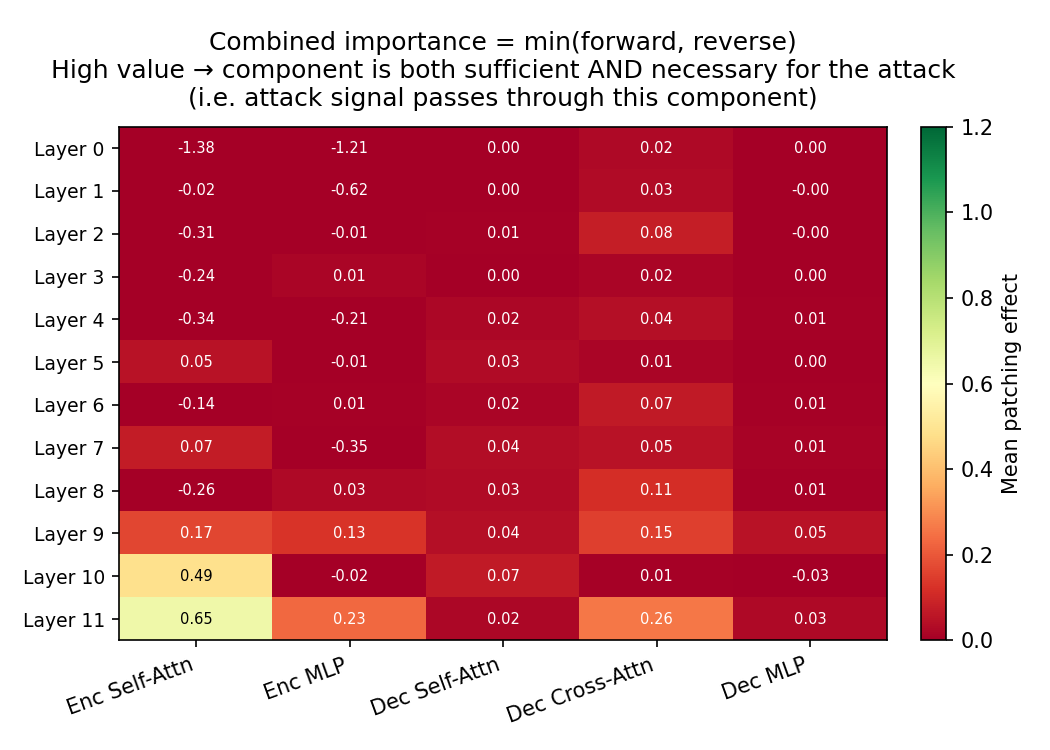
\includegraphics[width=0.75\textwidth]{outputs/plots/combined_layer_component_heatmap.png}
  \caption{Combined importance for a single worked example
  (\texttt{relevant\_start\_5}, the canonical attack used throughout this
  project, corrected data), shown here as concrete, single-attack proof
  that the fix produces genuinely differentiated components — compare
  \texttt{Enc Self-Attn} ($0.65$ at layer~11) against \texttt{Enc MLP}
  ($0.23$): close in the sense that both are elevated, but no longer
  identical the way the bug forced them to be. This one attack already
  shows the same qualitative story as the 105-attack aggregate
  (Figure~\ref{fig:aggcombined} below): encoder self-attention rises
  sharply in the last two layers and dominates every other component.}
  \label{fig:singleheatmap}
\end{figure}

\paragraph{A side effect worth flagging: early-layer sign-flipped
overshoot.} At layer~0, both \texttt{Enc Self-Attn} ($-1.38$) and
\texttt{Enc MLP} ($-1.21$) show large \emph{negative} combined effects —
patching this early layer's contribution pushes the score \emph{away} from
the attack direction, past the control baseline, rather than partway
toward the attack. This is not an artefact of the bug (both values are
independently computed and merely similar in magnitude, not identical);
it is the same qualitative phenomenon Experiment~6 documents in detail for
positional patching: an early-layer intervention is processed by many
subsequent layers before the final score is read out, and that additional
processing can amplify or invert an initially small perturbation. Late-layer
patching (layers~9--11) does not show this, since there are few or no
remaining layers left to compound the effect — consistent with why this
report's headline finding concentrates on late layers specifically.

% =====================================================================
\section{Results: Cross-Attack Comparison (105 Attacks)}
\label{sec:multi}
% =====================================================================

The multi-attack sweep covers 7 tokens
(\texttt{relevant, true, false, information, bar, important, relevance})
$\times$ 3 positions (\texttt{start, end, random}) $\times$ 5 repetition counts
$(1\ldots5)$, for 105 attacks; all 105 ran successfully and are aggregated in
\texttt{outputs/attack\_comparison/}. The shared-example intersection contains
487 pairs.

\subsection{Attack strength}

\begin{figure}[H]
  \centering
  
\includegraphics[width=0.95\textwidth]{outputs/attack_comparison/attack_strength_bar.png}
  \caption{Mean attack delta $\bar\Delta$ per attack. Taller bars are stronger
  attacks (larger score inflation).}
  \label{fig:bar}
\end{figure}

\paragraph{Interpretation.} Attack strength depends strongly on \emph{which token}
and \emph{where} it is injected, and grows with repetition count:
\begin{itemize}[nosep]
  \item \texttt{information\_start\_5} ($\bar\Delta=+0.381$),
        \texttt{relevant\_start\_5} ($+0.364$) and
        \texttt{relevant\_end\_5} are the \emph{strongest}: tokens that are
        semantically aligned with the relevance task push the score up the most,
        and stuffing them at the \texttt{start} with 5 repetitions maximises the
        effect (cf.\ \texttt{information\_start\_1}$=-0.112 \to$
        \texttt{information\_start\_5}$=+0.381$).
  \item \texttt{random}-position injections are mostly \emph{negative} (e.g.\
        \texttt{relevant\_random\_5}$=-0.287$): scattering the trigger inside the
        passage tends to \emph{lower} the score, because it disrupts the passage
        rather than presenting a clean relevance cue.
  \item Some tokens (\texttt{bar}, \texttt{true}, \texttt{false}) are weak or
        negative regardless of placement, showing the attack is not just ``more
        tokens'' but depends on semantic content.
\end{itemize}

\subsection{Component importance across attacks}

Figure~\ref{fig:aggcombined} summarises the whole sweep in a single compact map:
for each (layer, component) it shows the combined importance
$\min(\text{forward},\text{reverse})$, averaged across all 105 attacks. This is
the same layout as a per-attack heatmap, but every cell is now an average over
the entire grid of triggers, positions and repetition counts.

\begin{figure}[H]
  \centering
  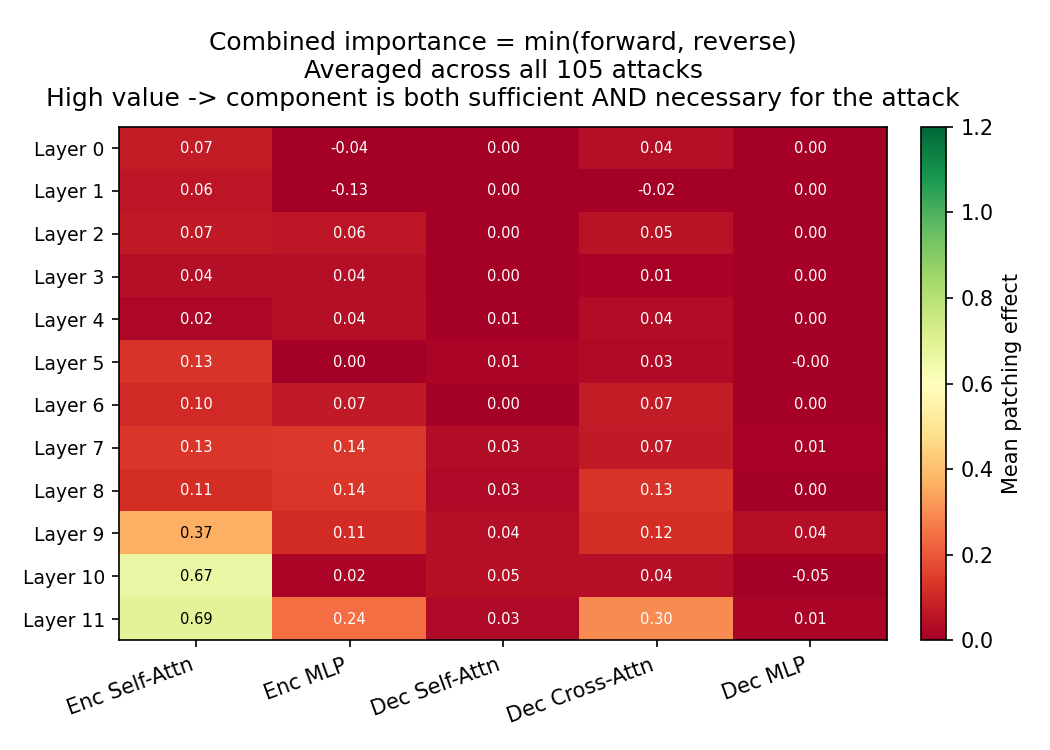
\includegraphics[width=0.7\textwidth]{outputs/attack_comparison/aggregate_combined_heatmap.png}
  \caption{\textbf{Aggregate combined importance} $=\min(\text{forward},
  \text{reverse})$, averaged across all 105 attacks. Rows are layers, columns
  are components. Bright $\Rightarrow$ the component is, on average, both
  sufficient \emph{and} necessary for the attack. The signal concentrates in
  \emph{encoder self-attention} at layers~9--11.}
  \label{fig:aggcombined}
\end{figure}

\paragraph{Interpretation.} The aggregate map confirms a single, consistent
pathway: encoder self-attention rises from $\approx0.37$ at layer~9 to
$\approx0.65$--$0.69$ at layers~10--11, dwarfing every decoder component and the
encoder MLP. The decision is built at the top of the \emph{encoder}, not in the
decoder.

\subsection{Per-attack heatmap matrix}

Figure~\ref{fig:heatmapmatrix} shows every attack at once: rows are
(token, position) groups, sub-rows within each are the three patching
directions (forward, reverse, combined), and columns are repetition
counts $1$--$5$. Bright cells indicate high normalised patching effect.
This is a single pre-stitched image (\texttt{scripts/make\_heatmap\_matrix.py}
compositing the same 315 per-attack PNGs that would otherwise need to be
included individually), chosen deliberately over embedding all 105
attacks' plots one figure at a time so that this report stays
self-contained and portable — compiling it elsewhere only requires this
one file, not the full \texttt{outputs/attacks/*/plots/} directory tree.

\begin{figure}[H]
  \centering
  \includegraphics[width=\textwidth]{outputs/attack_comparison/heatmap_matrix.png}
  \caption{All 105 attacks at once: rows are (token, position) groups
  (3 sub-rows each: forward/reverse/combined), columns are repetition
  counts 1--5. Zoom in digitally for individual cells — at print
  resolution this is an overview, not a substitute for
  Figure~\ref{fig:aggcombined}'s aggregate or the per-attack CSVs for
  precise numbers.}
  \label{fig:heatmapmatrix}
\end{figure}

\begin{figure}[H]
  \centering
  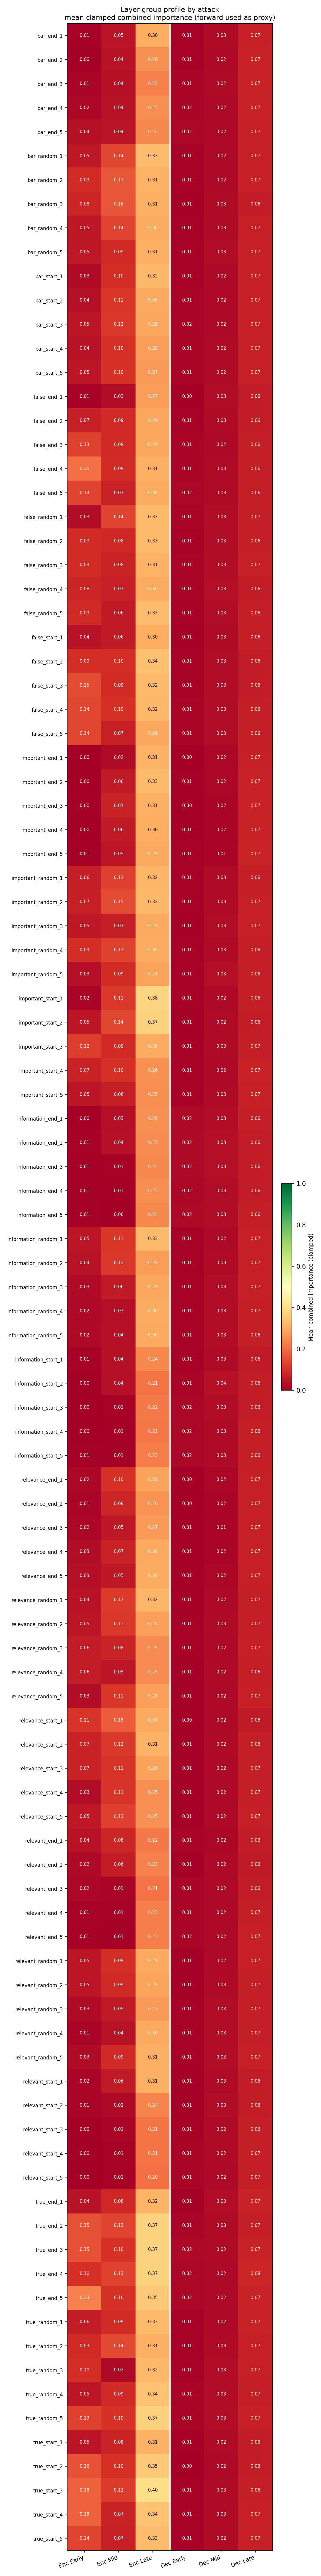
\includegraphics[width=0.95\textwidth]{outputs/attack_comparison/layer_profile_heatmap.png}
  \caption{Layer-wise importance profile per attack, showing where in depth each
  attack concentrates.}
  \label{fig:layerprof}
\end{figure}

\paragraph{Interpretation.} The cross-attack maps are remarkably consistent:
for \emph{every} one of the 105 attacks the \texttt{top\_component} is
\textbf{encoder self-attention}, peaking at the \textbf{final encoder layers}
(layer~11 for 70 attacks, layer~10 for 32, with only 3 outliers at layers~0/9).
The combined importance at the peak ranges from $0.49$ to $0.97$ (mean $0.73$).
Averaged over the late blocks the encoder is by far the dominant carrier
(mean late-encoder effect $0.29$) compared with decoder cross-attention
($0.15$), decoder self-attention ($0.035$) and decoder MLP ($0.017$). The
shared conclusion is that, \emph{regardless of the trigger word}, the spurious
relevance signal is built and concentrated in the \textbf{encoder's
self-attention} at the top of the encoder, where the injected tokens are mixed
into the passage representation; the decoder then reads this already-corrupted
representation, so the downstream decoder cross-attention carries only a weaker,
secondary share of the effect.

% =====================================================================
\section{Overall Interpretation and Discussion}
% =====================================================================

Taken together, the cross-attack results paint one coherent
mechanistic picture:

\begin{enumerate}
  \item \textbf{No single ``attack neuron''; a depth-cumulative pathway.} The
        injected relevance signal is not localised to one early component. It is
        built up gradually through the residual stream and only becomes a
        decision in the upper half of the network.
  \item \textbf{The late encoder is the locus of the decision.} Encoder
        self-attention in the final encoder blocks (layers 10--11) is
        simultaneously \emph{sufficient} and \emph{necessary}: it is where the
        injected tokens are mixed into the passage representation. The decoder
        cross-attention that subsequently reads this representation carries only
        a secondary share of the effect. The top of the encoder is therefore
        exactly where one would intervene to defend the ranker.
  \item \textbf{Attack success is semantic, not merely token-count.} Tokens
        aligned with the relevance task (\texttt{relevant}, \texttt{information})
        injected at the \texttt{start} and repeated five times are far more
        effective than random words or random positions; some placements even
        backfire.
  \item \textbf{Defensive implication.} Because the pathway is concentrated and
        consistent across attack types, monitoring or regularising the
        \emph{late-encoder self-attention} that integrates the injected tokens
        into the passage representation is a promising and targeted defence,
        rather than having to police every layer.
\end{enumerate}

% =====================================================================
\section{Limitations and Threats to Validity}
\label{sec:limits}
% =====================================================================

\begin{itemize}
  \item \textbf{Residual-stream granularity.} Patches act at sub-layer block
        outputs, so effects are cumulative; the method localises \emph{depth and
        broad component}, not individual attention heads or neurons.
  \item \textbf{Padded control.} The masked-prefix control is a careful but
        artificial baseline; absolute effect magnitudes are defined relative to
        it (Eq.~\ref{eq:delta}).
  \item \textbf{Sample size.} Patching uses up to 100 examples per attack (30 in
        the fast multi-attack sweep); means are stable but tails are noisy.
  \item \textbf{Single model / dataset.} Results are for monoT5-base on DL19;
        larger monoT5 variants (24 layers) would need the layer groups in
        \texttt{configs/default.yaml} adjusted.
\end{itemize}

% =====================================================================
\section{Reproducibility}
% =====================================================================

From the experiment directory, with the \texttt{advseq2seq} conda environment
(which provides \texttt{torch}, \texttt{transformers}, \texttt{matplotlib},
\texttt{pandas}, \texttt{numpy}, \texttt{pyyaml}):

\begin{lstlisting}
# Single-attack pipeline (stages 00-04)
python scripts/00_prepare_pairs.py
python scripts/01_score_and_select.py
python scripts/02_cache_activations.py
python scripts/03_run_layer_patching.py
python scripts/04_plot_results.py
python scripts/05_sanity_check_outputs.py   # read-only checks

# Multi-attack sweep + aggregation (stages 10-11)
python scripts/10_run_multi_attack_pipeline.py
python scripts/11_compare_attacks.py
\end{lstlisting}

\noindent Outputs are written under \texttt{outputs/} (single attack) and
\texttt{outputs/attacks/} + \texttt{outputs/attack\_comparison/} (multi-attack).

% =====================================================================
\section*{Appendix: Glossary of Key Quantities}
\addcontentsline{toc}{section}{Appendix: Glossary of Key Quantities}
% =====================================================================

\begin{description}[leftmargin=1.4em,style=nextline]
  \item[$\score$] $\operatorname{logit}(\texttt{true})-\operatorname{logit}(\texttt{false})$ at the first decoder step.
  \item[$\Delta$] $\score_{\text{attack}}-\score_{\text{control}}$ — the attack effect to be explained.
  \item[$\fwd_{L,C}$] forward effect, Eq.~\eqref{eq:fwd} — sufficiency of $(L,C)$.
  \item[$\rev_{L,C}$] reverse effect, Eq.~\eqref{eq:rev} — necessity of $(L,C)$.
  \item[combined] $\min(\fwd,\rev)$ — both sufficient and necessary.
  \item[Type A / B / C] original / padded-control / attacked inputs.
  \item[early / mid / late] layer groups 0--3 / 4--7 / 8--11.
\end{description}

\end{document}
